%% ----------------------------------------------------------------
%% Background.tex
%% ----------------------------------------------------------------
\chapter{Background and literature search}

There were lots of different algorithms existing in the field of object detection and tracking. Some of those algorithms were investigated in this project in order to identify a set of suitable algorithms that were both accurate and efficient enough to analysis video stream from camera in real-time.

Object tracking generally consists of 2 steps. Firstly, location and region of each object appeared in the frame need to be identified. Afterwards, tracking objects by analyse movement of each object in adjacent frames.

\section{Object identification}

Being able to detect objects in a video frame is the first, also the most important and challenging step to do object tracking. This is generally accomplished by separation of foreground objects and background image.

\subsection{Colour based}
\label{bgs:colour}

Colour can provide enough information of a specific object. For easier analysis of colour information, a hue-saturation-value (HSV) colourspace \cite[p.~301]{colourspace} representation converted from the original RGB colourspace is usually used, because it would be easier to filter a range of colour based on hue, saturation and brightness.

A simple colour based foreground mask can be generated easily by filtering target colour. For example, an simple implementation \cite{MOTBOC.git} based on colour filtering object detection, as shown in \fref{Figure:MOTBOC}.

\begin{figure}[H]
  \centering
  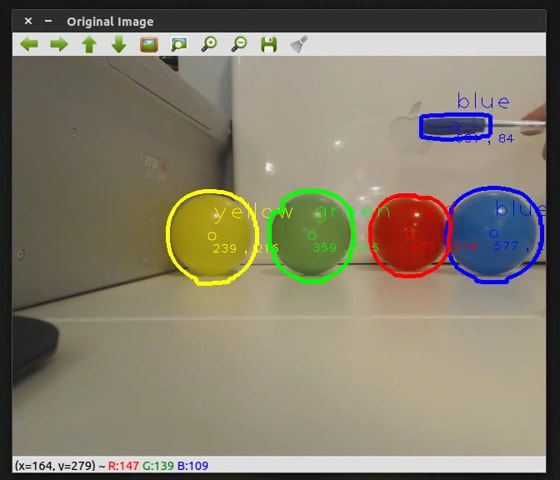
\includegraphics[width=0.6\columnwidth]{MOTBOC}
  \caption{Multi Object Tracking Based on Color (adapted from \cite{MOTBOC.git})}
  \label{Figure:MOTBOC}
\end{figure}

This implementation does not require a lot of computation, thus was very fast, could be suitable for robots that are tracking sonething like a single coloured ball or piece of paper, also could be useful for line racing car projects.

There were also researches using a more complex particle filtering algorithm based on colour distributions, such as \cite{nummiaro2003color}, shown by \fref{Figure:nummiaro2003color}.

\begin{figure}[H]
  \centering
  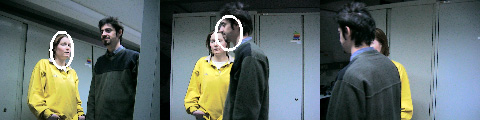
\includegraphics[width=0.9\columnwidth]{colour_based}
  \caption{Object detection based on colour distribution particle filtering (adapted from \cite{nummiaro2003color})}
  \label{Figure:nummiaro2003color}
\end{figure}

However, if there were other targets with similar colour, the algorithm may failed to distinguish them, as shown by the second image in \fref{Figure:nummiaro2003color}. It also requires a specific model associated with each of the objects to be tracked.

\subsection{Shape based}

Another important information about an object is its shape. By extracting object edges in the scene than apply appropriate shape transformation and filtering algorithms, an object could also be detected based on its shape.

\fref{Figure:circles} shows the image processed by circle detection, based on OpenCV's implementation of Hough Circle Transform \cite{opencv:hough_circle}. The frame captured from camera (\fref{Figure:edges:original}), was converted to gray scale and blurred first, as shown in \fref{Figure:edges:blur}. Blur, or smooth was often necessarily to reduce possibly false object edges that might be detected. Afterwards the object edges in the image was extracted as in \fref{Figure:edges:edges}. Finally \fref{Figure:edges:circles} shows the circles detected by the algorithm.

\begin{figure}[H]
  \centering
  \subfigure [] {
    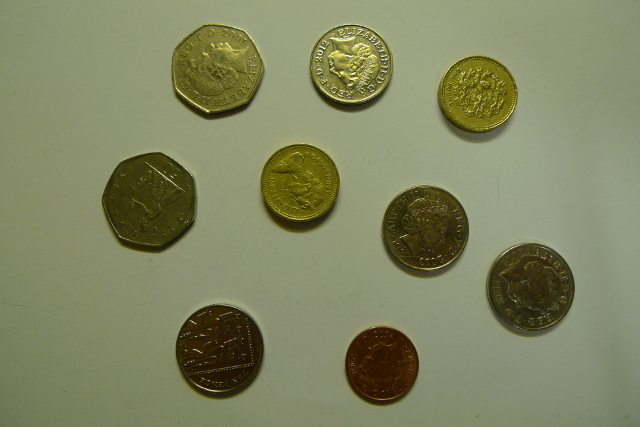
\includegraphics[width=0.45\columnwidth]{simple_original}
    \label{Figure:edges:original}
  }
  \subfigure [] {
    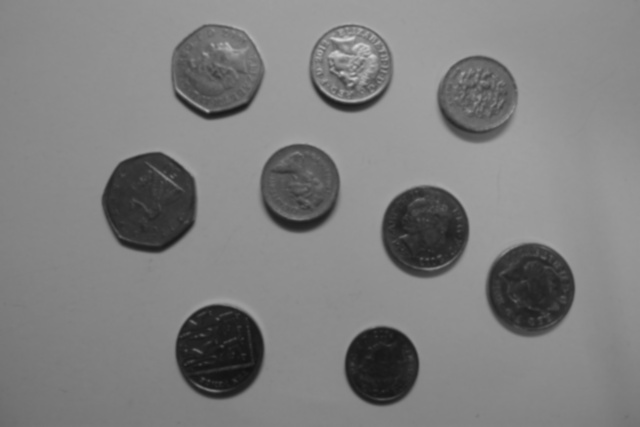
\includegraphics[width=0.45\columnwidth]{simple_blur}
    \label{Figure:edges:blur}
  }
  \subfigure [] {
    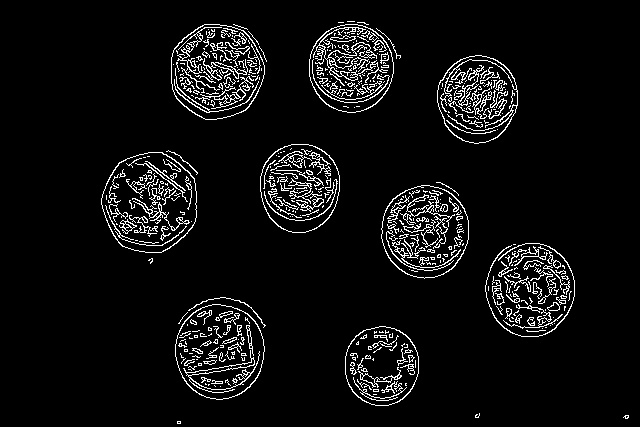
\includegraphics[width=0.45\columnwidth]{simple_edges}
    \label{Figure:edges:edges}
  }
  \subfigure [] {
    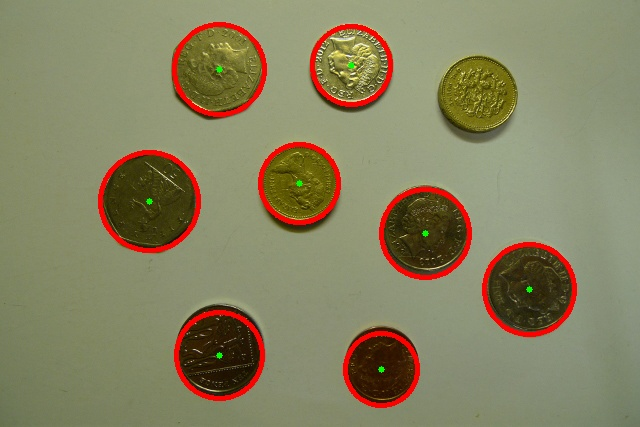
\includegraphics[width=0.45\columnwidth]{simple_circles}
    \label{Figure:edges:circles}
  }
  \caption{Circle detection. \subref{Figure:edges:original} The original image, \subref{Figure:edges:blur} image converted to gray scale and blurred, \subref{Figure:edges:edges} edges detected, \subref{Figure:edges:circles} circles detected}
  \label{Figure:circles}
\end{figure}

This implementation could be suitable for ball tracking purpose. By combining with the simple colour filtering algorithm as described in Section \ref{bgs:colour}, a single coloured ball could be efficiently tracked.

\subsection{Cascade Classifier}

Cascade classifier \cite{cascade} is another widely used technique. It concatenates several classifiers detecting different object features to finally recognise objects, and its accuracy can be improved by training the classifier both positively and negatively. It was usually used not only for object detection, but also for object classification, for example recognise human and different classes of vehicles in a single frame.

The OpenCV's cascade classifier implementation \cite{opencv:cc} of face and eye detection was investigated as shown in \fref{Figure:cc_face}.

\begin{figure}[H]
  \centering
  \includegraphics[width=0.6\columnwidth]{"CC face"}
  \caption{Face and eye detection cascade classifiers, detected face was circled by pink, whereas detected eyes were circled by blue}
  \label{Figure:cc_face}
\end{figure}

\subsection{Motion based background subtraction}
\label{motion_bs}

By differenceing current frame and previous frames then probably build up a background model image, it is also possible to detect moving objects efficiently. The BGSLibrary \cite{bgslibrary} is specifically developed for this purpose, it offers 37 different background substraction algorithms implemented using OpenCV, published under GNU GPL v3 license.

This type of algorithms suit well for static camera movement tracking, and were not limited by objects' geometry shapes, therefore was used in this project.

\subsection{Connected component analysis}
\label{blob}

After obtained the foreground object mask by background subtraction (Section \ref{motion_bs}), it need to be interpreted as objects, so that the properties of each object can then be retrieved, including shape, bounding rectangle and location of the object.

Connected component analysis, or Connected component labeling, is used for detecting connected regions (blobs), which are the possible regions of objects. A blob detector can be used to mark and label individual objects from the foreground mask, therefore obtain parameters such as shape, size, location and orientation of the object.

There were also lots of free and open source blob detection libraries available, e.g. the simple blob detector came with OpenCV \cite{opencv:blob}, cvBlob library \cite{cvblob}.

\section{Movement tracking}
\label{bg:tracking}

After determined bounding rectangle, or region of interest (ROI), of an object by methods described above, the object then can be tracked between adjacent frames. Movement parameter such as velocity and acceleration may also be obtained by physical modelling of the objects.

\subsection{Meanshift}

Meanshift \cite{fukunaga2013introduction} is an algorithm used to track the movement of a fixed size ROI window between adjacent frames, by finding the peak of probability distribution of the ROI from the new frame. It can be easily implemented with OpenCV \cite{opencv:camshift}.

\subsection{Continuously Adaptive Meanshift}

Continuously Adaptive Meanshift (CAMshift) \cite{bradski1998computer} is an algorithm based on Meanshift algorithm, that can handle target object size changing and rotation by iterating over the ROI to find the most suitable configuration. This algorithm can also be easily implemented using OpenCV \cite{opencv:camshift}, and was used by lots of researches for tracking purpose, such as \cite{chu2007object}, \cite{xu2012moving} and \cite{nouar2006improved}.

\section{Object recognition}

Object recognition could also be developed by applying different cascade classifiers to the ROI of the specific object. This process is the most computation intensive and time consuming step, therefore should be executed as few as possible to achieve maximum power saving, for example, only execute once when the object first enter the sense or at its maximum visible size to the camera.

\section{Automatic feedback control}

Research about energy-efficient object detection by utilising hardware-level operations exists \cite{casares2011energy}, achieved an energy consumption reduction by $54.136\%$. But it was done on a very different and limited platform, also possible to extend further.
